\documentclass[10pt]{article}
% Include statements
\usepackage{graphicx}
\usepackage{amsfonts,amssymb,amsmath,amsthm}
\usepackage[numbers,square]{natbib}
\usepackage[left=1in,top=1in,right=1in,bottom=1in,nohead]{geometry}
\usepackage[all]{xy}
\usepackage{multirow,rotating,array}
\usepackage[ruled,lined]{algorithm2e}
\SetKw{KwSet}{Set}
\usepackage{pdfsync}
\usepackage{setspace}
\usepackage{bbm}
\usepackage{hyperref}
\hypersetup{backref,colorlinks=true,citecolor=blue,linkcolor=blue,urlcolor=blue}
\renewcommand{\qedsymbol}{$\blacksquare$}
\setlength{\parindent}{0cm}
\setlength{\parskip}{10pt}
\bibliographystyle{mybibsty}

%%%%%%%%%%%%%%%%
%% I added this (charlie)
\usepackage{breqn}
%% this allows to break long fourier expansions onto multiple lines

%%this gives you an equality sign with the word 'def' on top of it
\newcommand\myeq{\stackrel{\normalfont\mbox{def}}{=}}
%%%%%%%%%%%%%%%%%

% Theorem environments (\autoref compatible)
\usepackage{aliascnt}

\newtheorem{theorem}{Theorem}[section]

\newaliascnt{result}{theorem}
\newtheorem{result}[theorem]{Result}
\aliascntresetthe{result}
\providecommand*{\resultautorefname}{Result}
\newaliascnt{lemma}{theorem}
\newtheorem{lemma}[lemma]{Lemma}
\aliascntresetthe{lemma}
\providecommand*{\lemmaautorefname}{Lemma}
\newaliascnt{prop}{theorem}
\newtheorem{proposition}[prop]{Proposition}
\aliascntresetthe{prop}
\providecommand*{\propautorefname}{Proposition}
\newaliascnt{cor}{theorem}
\newtheorem{corollary}[cor]{Corollary}
\aliascntresetthe{cor}
\providecommand*{\corautorefname}{Corollary}
\newaliascnt{conj}{theorem}
\newtheorem{conjecture}[conj]{Conjecture}
\aliascntresetthe{conj}
\providecommand*{\conjautorefname}{Corollary}
\newaliascnt{def}{theorem}
\newtheorem{definition}[def]{Definition}
\aliascntresetthe{def}
\providecommand*{\defautorefname}{Definition}
\newaliascnt{ex}{theorem}
\newtheorem{example}[ex]{Example}
\aliascntresetthe{ex}
\providecommand*{\exautorefname}{Example}


\newtheorem{assumption}{Assumption}
\renewcommand{\theassumption}{\Alph{assumption}}
\providecommand*{\assumptionautorefname}{Assumption}

\def\algorithmautorefname{Algorithm}
\renewcommand*{\figureautorefname}{Figure}%
\renewcommand*{\tableautorefname}{Table}%
\renewcommand*{\partautorefname}{Part}%
\renewcommand*{\chapterautorefname}{Chapter}%
\renewcommand*{\sectionautorefname}{Section}%
\renewcommand*{\subsectionautorefname}{Section}%
\renewcommand*{\subsubsectionautorefname}{Section}% 


% My Macros
\def\indep{\perp\!\!\!\perp}
\newcommand{\given}{\mbox{ }\vert\mbox{ }}
\newcommand{\F}{\mathcal{F}}
\newcommand{\Expect}[1]{\mathbb{E}\!\left[#1\right]}
\renewcommand{\P}{\mathbb{P}}
\newcommand{\R}{\mathbb{R}}
\newcommand{\X}{\mathcal{X}}
\newcommand{\B}{\mathcal{B}}
\DeclareMathOperator*{\Variance}{Var}
\newcommand{\Var}[1]{\Variance\!\left[#1\right]}
\DeclareMathOperator*{\Covariance}{Cov}
\newcommand{\Cov}[1]{\Covariance\!\left[#1\right]}
\newcommand{\Y}{\mathcal{Y}}
\newcommand{\norm}[1]{\left|\left| #1 \right|\right|}
\newcommand{\email}[1]{\href{mailto:#1}{#1}}
\DeclareMathOperator*{\argmin}{argmin}
\newcommand{\indicator}[2]{\mathbbm{1}_{#1}(#2)}
\newcommand{\cdist}{\rightsquigarrow}
\newcommand{\cprob}{\xrightarrow{P}}
\newcommand{\clp}{\xrightarrow{L_p}}
\newcommand{\cas}{\xrightarrow{as}}
\renewcommand{\bar}{\overline}

% Your new macros
\newcommand{\sbullet}{\,\begin{picture}(1,1)(0,-3)\circle*{3}\end{picture}\ }
\DeclareMathOperator{\Bias}{Bias}


% To be entered
\newcommand{\lecture}{Prof.\ Homrighausen}
\newcommand{\scribe}{Chuck Vollmer}
\newcommand{\chtitle}{Linear Models}
\newcommand{\lecdate}{August 27th, 2014}


\begin{document}
\rule{6.5in}{1pt}

\textsc{Statistical Machine Learning
  \hfill 4 --- \chtitle
  \hfill \lecdate}

\textsc{Lecturer: \lecture \hfill Scribe: \scribe}
\rule{6.5in}{1pt}


\section{Parseval's Theorem}


If a function has a Fourier series given by 

\begin{dmath}
f(x)=\frac{1}{2}a_0+\sum_{n=1}^{\infty}{a_n\cos(nx)+\sum_{n=1}^{\infty}b_n\sin(nx)}
\end{dmath}


then Bessel's inequality becomes an equality know as {\em Parseval's theorem}, from (1):

\begin{dmath}
 [f(x)]^2 = 
 \frac{1}{4}a_0^2 + a_0 \sum_{n=1}^{\infty}{a_n\cos(nx)+b_n\sin(nx)} \\ 
 + \sum_{n=1}^{\infty} \sum_{m=1}^{\infty} {a_na_m\cos(nx)\cos(mx)+a_nb_m\cos(nx)\sin(mx) \\
 +a_mb_n\sin(nx)\cos(mx)+b_nb_m\sin(nx)\sin(mx)}
 \end{dmath}

Integrating

\begin{dmath}
\int_{-\pi}^{\pi}[f(x)]^2dx = \frac{1}{4}a_0^2\int_{-\pi}^{\pi}dx+a_0\int_{-\pi}^{\pi}\sum_{n=1}^{\infty}{a_n\cos(nx)+b_n\sin(nx)}dx+\int_{-\pi}^{\pi}\sum_{n=1}^{\infty}\sum_{m=1}^{\infty}{a_na_m\cos(nx)\cos(mx)+a_nb_m\cos(nx)\sin(mx)+a_mb_n\sin(nx)\cos(mx)+b_nb_m\sin(nx)\sin(mx)}dx 
=\frac{1}{4}a_0^2(2\pi)+0+\sum_{n=1}^{\infty} \sum_{m=1}^{\infty}{a_na_m\pi \delta_{nm}+0+0+b_n b_m \pi \delta_{nm}}
\end{dmath}


So

\begin{dmath}
\frac{1}{\pi} \int_{-\pi}^{\pi}[f(x)]^2dx=\frac{1}{2}a_0^2+\sum_{n=1}^{\infty}(a_n^2+b_n^2)
\end{dmath}

\newpage

\begin{example}
Thus, under our conditions the problem is well-understood if the error of the representation is measured using the Euclidean or $\ell_2$ norm. Since the $\ell_2$ norm is preserved under rotations, by Parseval's theorem, we have

\begin{dmath}
\|f-\hat{f} \|_2^2 = \sum_i {(f_i - \sum_k{\beta_k \phi_k})^2} = \sum_i {(<f,\phi_k> - \beta_k)^2}
\end{dmath}

and it is clear that the solution under this error measure is to retain the largest K inner products $<f, \phi_k>$, which are also the coefficients of the basis expansion of $f$. 

\end{example}






\section{Vandermonde Matrix}

A {\em Vandermonde Matrix} - of order $n$- is of the form

\begin{dmath}
\left(
	\begin{array}{ccccc}
	1 &x_1 & x_1^2 & \cdots & x_1^{n-1} \\
	1& x_2 & x_2^2 & \cdots & x_2^{n-1} \\
	\vdots & \vdots & \vdots & \ddots & \vdots \\
	1& x_n & x_n^2 & \cdots & x_n^{n-1}
	\end{array} \right)
\end{dmath}

A Vandermonde Matrix is a type of matrix that arises in the polynomial least squares fitting, Lagrange interpolating polynomials (Hoffman and Kunze p. 114), and the reconstruction of a statistical distribution from the distribution's moments (von Mises 1964; Press et al. 1992, p. 83). 

\bigskip

Notes:

\begin{itemize}
	\item Some authors define the transpose of this matrix as the Vandermonde matrix.
	\item The solution of an $n \times n$ Vandermonde matrix equation requires  $O(n^2)$ operations.
	\item The determinants of Vandermonde matrices have a particularly simple form.
\end{itemize}





%%%%%%%%%%
\section{Spectral (operator) Norm}

The {\em operator norm} of a linear operator $\mathbf{T}:\mathbf{V} \rightarrow \mathbf{W}$ is the largest value by which $\mathbf{T}$ stretches an element of $\mathbf{V}$,

\begin{dmath}
\|T\| = \sup_{\|v\|=1}\|T(v)\|
\end{dmath}

It is necessary for V and W to be normed vector spaces. The operator norm of a composition is controlled by the norms of the operators,

\begin{dmath}
\|TS\| \leq \|T\| \|S\|
\end{dmath}

When $\textbf{T}$ is given by a matrix, say $\mathbf{T}(v)=\mathbf{A}v$, then $||T||$ is the square root of the largest eigenvalue of the symmetric matrix $A^TA$, all of whose eigenvalues are nonnegative.  So, if we have the following linear operator

\begin{example}
So, if we have the following linear operator
\begin{dmath}
A = \left(
	\begin{array}{ccc}
	2&0 & 0 \\
	3 & 0 & 2
	\end{array} \right) 
\end{dmath}

Then, we find the following 
\begin{dmath}
A^T A = \left(
	\begin{array}{ccc}
	13 & 0 & 6 \\
	0 & 0 & 0 \\
	6 & 0 & 4
	\end{array} \right)
\end{dmath}
which has eigenvalues $\{0,1,16\}$, so $\|A\| = 4$.
\end{example}












\section{Kullback-Leibler Divergence}

It is interesting to note a few things about this pseudo-metric: the Kullback-Leibler Discrepancy (KLD).

\begin{enumerate}
	\item the KLD can be seen as a measure of statistical independence
	\item a Pythagorean Theorem exists in which the KLD plays a role similar to that of squared distance in Euclidean Geometry
\end{enumerate}

\subsection{a measure of independence}

This can easily be seen by measuring the KLD from the distribution of $P(Y)$ of $Y$ to the product of its marginal distributions:

\begin{dmath}
I(Y) \myeq K[P(Y), \Pi_i P(Y_i)]
\end{dmath}

where the divergence K[Q,R] is defined as in the class notes:

\begin{dmath}
K[Q,R] \myeq \int_Y {Q(y) \log \frac{Q(y)}{R(y)}} dy
\end{dmath}



\subsection{KLD Pythagorean Theorem}

Now, another interesting feature is how the KLD plays a role similar to the squared distance in Euclidean Geometry.

\begin{theorem}
For an exponential family, $E$, of distributions and for any P (not necessarily in $E$), there is a unique distribution $\mathcal{Q}$ of $E$ such that the divergence from P to any distribution R of $E$ decomposes as
\begin{dmath}
K[P,R] = K[P,Q] + K[Q,R].
\end{dmath}
\end{theorem}

This Theorem is illustrated below:


\begin{figure}[h]
\begin{center}
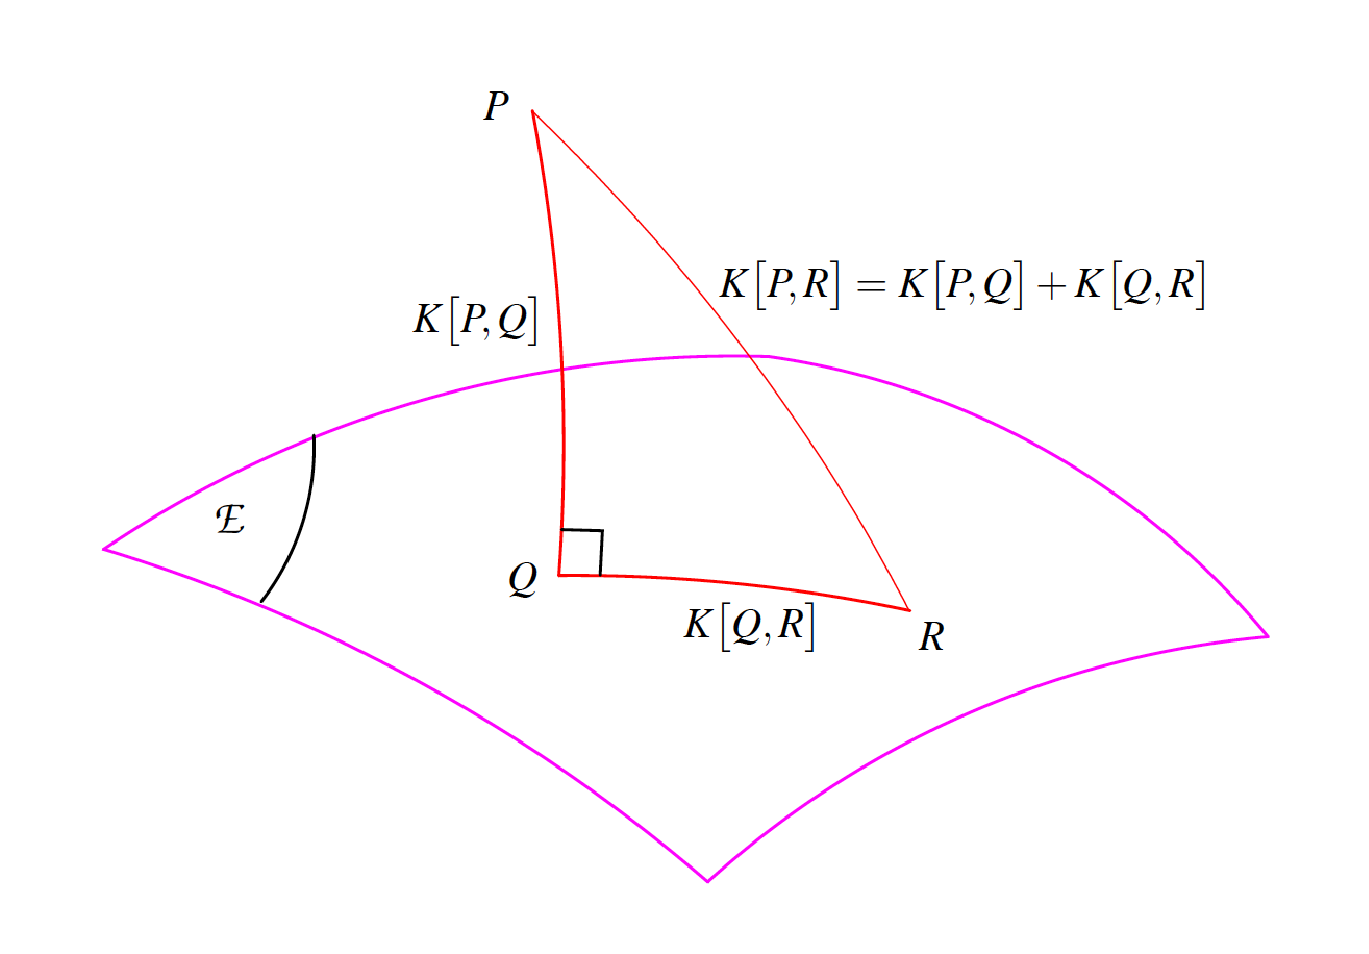
\includegraphics[scale=0.50]{KLD.pdf}
\end{center}
\end{figure}

This decomposition shows that Q is the closest distribution to P in E in the KLD sense since K[Q,R] reaches its minimum value of 0 for Q = R. Thus, Q can be called the ``orthogonal projection" of P onto E and decomposition (13) should be read as a Pythagorean theorem in distribution space with the KL divergence being the analogue of a squared Euclidean distance.  

And remember, since the divergence is not a true distance the Pythagorean theorem is actually a point-to-point relation.



\newpage


\section{KLD and the AIC}

Akaike (1973) showed firstly that the maximized log-likelihood is biased upward as an estimator of the model selection criterion. Second, he showed that under certain conditions (these conditions are important, but quite technical), that this bias is approximately equal to K, the number of estimable parameters in the approximating model. Thus, an approximately unbiased estimator of the relative, expected K-L information is

\begin{dmath}
\mathbb{P}_f[\log(g(Y;\theta))] \approx \log(g(Y;\hat{\theta}_{ML})) -K
\end{dmath}

which thus gives us that

\begin{dmath}
-\mathbb{P}[\log(g(Y;\hat{\theta}_{ML}))] \approx -\log(g(Y;\hat{\theta}_{ML}))  + K
\end{dmath}

Akaike (1973) then defined "$an$ information criterion" (AIC) -in his words- "taking historical reasons into account" by multiplying by 2 to finally get

\begin{center}
\textbf{AIC} = $-2 \log(g(Y;\hat{\theta}_{ML})) + 2| \hat{\beta}_{ML} |$
\end{center}


\end{document}
